% This tells the program how to initially format my document.
\documentclass{article}

% List of packages to be included for the use of special commands and symbols.
\usepackage{amsmath,amssymb,amsthm}
\usepackage{mathtools}
\usepackage{mathrsfs}
\usepackage[letterpaper,margin=1in]{geometry}
\usepackage{enumitem}
%% remove ligatures (e.g. ``ff") to allow text copying from PDF
\usepackage{microtype}
\DisableLigatures{encoding = *, family = * }
\usepackage{fancyhdr}
\usepackage[T1]{fontenc}
\usepackage{lmodern}
\usepackage[USenglish]{babel}

\usepackage{tikz}
\usepackage{float}

\setlength{\parindent}{0cm}

\pagestyle{fancy}
\rhead{\large Alexander Novotny}
\lhead{\large CS 485 PA1}
\setlength{\headheight}{14pt}

\title{Stat 461 Programming Assignment 1}
\date{March 4, 2019}
\author{Alexander Novotny}

\begin{document}
\pagenumbering{roman}

\maketitle

\section*{Problem 1}
\subsection*{Approach}
As discussed in the assignment, we wish to solve a set of equations defined by an affine transformation:
\begin{align*}
	\hat{P}_1 &= AP_1 + b,\\
	\hat{P}_2 &= AP_2 + b,\\
	\hat{P}_3 &= AP_3 + b,\\
	\hat{P}_4 &= AP_4 + b,\\
\end{align*}
where $(P_1, P_2, P_3, P_4)$ are the original eye, nose, and mouth locations (found by hand) and $(\hat{P}_1, \hat{P}_2, \hat{P}_3, \hat{P}_4)$ are their fixed goal locations in the normalised images. This system can be reduced to an equivalent system
\begin{align*}
	\hat{p}_x &= Pc_1,\\
	\hat{p}_y &= Pc_2,\\
\end{align*}
where
\begin{align*}
	\hat{p}_x &= \begin{bmatrix}\hat{X}_1\\\hat{X}_2\\\hat{X}_3\\\hat{X}_4\end{bmatrix}, &
	\hat{p}_y &= \begin{bmatrix}\hat{Y}_1\\\hat{Y}_2\\\hat{Y}_3\\\hat{Y}_4\end{bmatrix}, &
	c_1 &= \begin{bmatrix}a_{11}\\a_{12}\\b_1\end{bmatrix}, &
	c_2 &= \begin{bmatrix}a_{21}\\a_{22}\\b_2\end{bmatrix},
\end{align*}
and
\[
	P =
	\begin{bmatrix}
		X_1 & Y_1 & 1\\
		X_2 & Y_2 & 1\\
		X_3 & Y_3 & 1\\
		X_4 & Y_4 & 1
	\end{bmatrix}.
\]

Unfortunately, since this an overdetermined system, an exact solution is unlikely to exist. So we find the closest (least squares) solution using Singular Value Decomposition (SVD) and back-substitution. This lets us construct $\tilde{A}$ and $\tilde{b}$ from our least squares solutions $\tilde{c}_1, \tilde{c}_2$ and acquire a close enough affine transformation
\[
	\hat{P} \approx \tilde{A}P + \tilde{b},
\]
for all of our fixed points.

\begin{figure}
	\begin{tikzpicture}
		\node[anchor=south west,inner sep=0] (image) at (0,0) {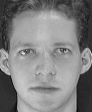
\includegraphics[width=.1\textwidth]{Sample1-1.png}};
		\begin{scope}[x={(image.south east)},y={(image.north west)}]
			\draw[red,ultra thick,rounded corners] (0.62,0.65) rectangle (0.78,0.75);
		\end{scope}
	\end{tikzpicture}
\end{figure}

\end{document}